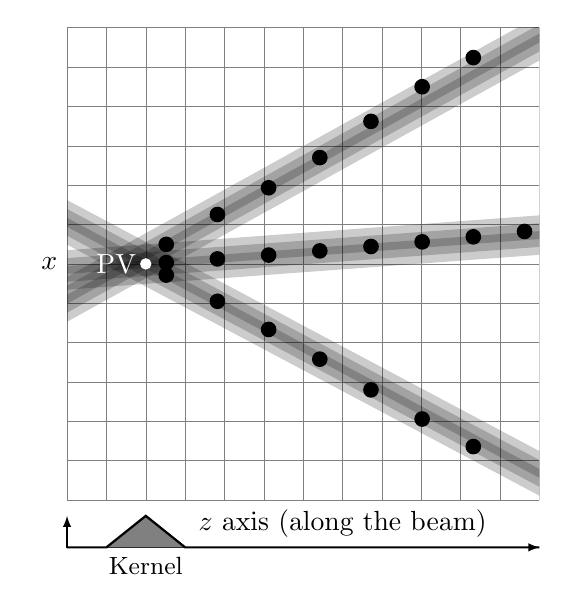
\begin{tikzpicture}[
    hit/.style={inner sep=2pt, fill, circle, black},
    simitrack/.style={shorten >= -6cm, shorten <= -6cm, opacity=.2, line width=.1cm,
        preaction={draw, line width=.3cm, opacity=.2},
        preaction={draw, line width=.5cm, opacity=.2}},
    bluesimitrack/.style={thick, blue,
        preaction={shorten >= -6cm, shorten <= -6cm, draw, opacity=.2, line width=.1cm,
            preaction={draw, blue, line width=.3cm, opacity=.2},
            preaction={draw, blue, line width=.5cm, opacity=.2}}}
        ]

    \path [use as bounding box] (-1.5,-3.8) rectangle (5,3);

    \node at (2.5,-3) [below] {$z$ axis (along the beam)};
    \node at (-1, 0) [left] {$x$};


        \begin{scope}[yshift=-3.6cm]
            \draw [latex-latex] (-1,.4) -- (-1,0) -- (5,0);
            \draw [thick, black, fill=gray]
                (-1,0) -- (-.5,0) -- (0,.4) -- (.5, 0) -- (5,0);
            \node at (0,0) [below] {\small Kernel};
        \end{scope}

    \clip (-1,-3) rectangle (5,3);

    \begin{scope}[xscale=.65, xshift=-.6cm]

        % def f(name, slope, factor):
        %     v = np.arange(1,9)
        %     vv = (v-.5)*slope + .05*np.sin(v*factor)
        %     q = np.linspace(.5, 8, 400)
        %     qq = (q-.5)*slope + .05*np.sin(q*factor)
        %     print(f'% {name} slope={slope} factor={factor}')
        %     for a,b in zip(v,vv):
        %         print(f'\coordinate ({name}{a}) at ({a}, {b:.3});')
        %     print()
        %     return q, qq, v, vv


        % (v-.5)*slope + .05*np.sin(v*factor)
        % A slope=0.4 factor=-5
        \coordinate (A7) at (1, 0.248);
        \coordinate (A6) at (2, 0.627);
        \coordinate (A5) at (3, 0.967);
        \coordinate (A4) at (4, 1.35);
        \coordinate (A3) at (5, 1.81);
        \coordinate (A2) at (6, 2.25);
        \coordinate (A1) at (7, 2.62);

        % B slope=0.06 factor=6
        \coordinate (B8) at (1, 0.016);
        \coordinate (B7) at (2, 0.0632);
        \coordinate (B6) at (3, 0.112);
        \coordinate (B5) at (4, 0.165);
        \coordinate (B4) at (5, 0.221);
        \coordinate (B3) at (6, 0.28);
        \coordinate (B2) at (7, 0.344);
        \coordinate (B1) at (8, 0.412);

        % C slope=-0.35 factor=7
        \coordinate (C7) at (1, -0.142);
        \coordinate (C6) at (2, -0.475);
        \coordinate (C5) at (3, -0.833);
        \coordinate (C4) at (4, -1.21);
        \coordinate (C3) at (5, -1.6);
        \coordinate (C2) at (6, -1.97);
        \coordinate (C1) at (7, -2.32);

    \end{scope}


    \draw[step=.5, gray, very thin, use as bounding box] (-1,-3) grid (5,3);

    \draw [simitrack] (A5) -- (A7) ;
    \draw [simitrack] (B6) -- (B8) ;
    \draw [simitrack] (C5) -- (C7) ;

    \draw [fill,white] (0,0) circle (.065) node [left] {PV};

    \node [hit] at (A1) {};
    \node [hit] at (A2) {};
    \node [hit] at (A3) {};
    \node [hit] at (A4) {};
    \node [hit] at (A5) {};
    \node [hit] at (A6) {};
    \node [hit] at (A7) {};

    \node [hit] at (B1) {};
    \node [hit] at (B2) {};
    \node [hit] at (B3) {};
    \node [hit] at (B4) {};
    \node [hit] at (B5) {};
    \node [hit] at (B6) {};
    \node [hit] at (B7) {};
    \node [hit] at (B8) {};

    \node [hit] at (C1) {};
    \node [hit] at (C2) {};
    \node [hit] at (C3) {};
    \node [hit] at (C4) {};
    \node [hit] at (C5) {};
    \node [hit] at (C6) {};
    \node [hit] at (C7) {};

\end{tikzpicture}
